\documentclass{beamer}
\usetheme{Warsaw}

\usepackage[utf8]{inputenc} 
\usepackage[french]{babel}		% pour une mise en forme "francaise"
\usepackage{amsmath,amssymb,amsthm}	% pour les maths
\usepackage{graphicx}			% pour inclure des graphiques
\usepackage{hyperref}			% si vous souhaitez que les references soient des hyperliens
\usepackage{color}			% pour ajouter des couleurs dans vos textes
\usepackage{parskip}
\usepackage{float}
\usepackage[T1]{fontenc}
\usepackage{graphicx}
\usepackage{stmaryrd}
\usepackage{tkz-tab}
\usepackage{pgfplots}
\usepackage{algorithm}
\usepackage[noend]{algpseudocode}

\def \dd {\mathrm{d}}
\def \E {\mathbb{E}}
\def \P {\mathbb{P}}


\title{Barrages et Risques d'Inondation}
\author{Zian Chen \& Ruikai Chen}	
\date{31 mai 2024}
\begin{document}
\frame{\titlepage}
\begin{frame}
\frametitle{Sommaire}
\tableofcontents
\end{frame} % 目录
\section{Introduction}
\begin{frame}{Introduction}
    Un barrage est un ouvrage artificiel ou naturel, établi en travers du lit
d'un cours d'eau, retenant ou pouvant retenir de l'eau. Les barrages ont plusieurs fonctions, par exemple : la régulation de cours d'eau; l'irrigation des cultures; la lutte contre les incendies, etc. La rareté des accidents est le résultat d'efforts attentifs depuis un siècle.
\end{frame}

\begin{frame}{Modélisation}
\begin{center}
\tikzset{every picture/.style={line width=0.75pt}} 
\begin{tikzpicture}[x=0.75pt,y=0.75pt,yscale=-1,xscale=1]
\draw  [draw opacity=0][fill={rgb, 255:red, 80; green, 227; blue, 226 }  ,fill opacity=1 ] (394.14,184.04) .. controls (394.14,192.76) and (387.07,199.84) .. (378.34,199.84) -- (229.82,199.87) .. controls (221.09,199.87) and (214.02,192.8) .. (214.02,184.07) -- (214.01,120.86) .. controls (214.01,120.86) and (214.01,120.86) .. (214.01,120.86) -- (394.13,120.83) .. controls (394.13,120.83) and (394.13,120.83) .. (394.13,120.83) -- cycle ;
\draw  [color={rgb, 255:red, 0; green, 0; blue, 0 }  ,draw opacity=1 ] (394.14,180.84) .. controls (394.14,191.33) and (385.63,199.84) .. (375.14,199.84) -- (233.02,199.87) .. controls (222.53,199.87) and (214.02,191.36) .. (214.02,180.87) -- (214,104.85) .. controls (214,104.85) and (214,104.85) .. (214,104.85) -- (394.13,104.82) .. controls (394.13,104.82) and (394.13,104.82) .. (394.13,104.82) -- cycle ;
\draw  [dash pattern={on 4.5pt off 4.5pt}]  (214.01,120.86) -- (394.13,120.83) ;
\draw   (189.37,219.96) -- (191.62,204.2) -- (195,207.63) -- (208.53,194.27) -- (215.31,201.13) -- (201.78,214.49) -- (205.17,217.92) -- cycle ;
\draw   (218.63,94.19) -- (202.74,93.2) -- (205.89,89.55) -- (191.51,77.12) -- (197.81,69.83) -- (212.2,82.25) -- (215.35,78.61) -- cycle ;
\draw   (444.56,71.48) -- (423.69,91.52) -- (404.26,99.14) -- (412.65,80.03) -- (433.52,59.99) -- cycle ;
\draw   (406.36,195.8) -- (424.86,218.05) -- (431.07,237.98) -- (412.61,228.24) -- (394.11,205.99) -- cycle ;
\draw (186,112.4) node [anchor=north west][inner sep=0.75pt]    {$X_{t}$};
\draw (107,51.4) node [anchor=north west][inner sep=0.75pt]    {$U_{n} \delta ( t=T_{n})$};
\draw (161,213.4) node [anchor=north west][inner sep=0.75pt]    {$rX_{t}$};
\draw (439,26.4) node [anchor=north west][inner sep=0.75pt]    {$\displaystyle A_{t} =\sum _{n=1}^{N_{t}} U_{n}$};
\draw (429,214.4) node [anchor=north west][inner sep=0.75pt]    {$\displaystyle \int _{0}^{t} rX_{s}\mathrm{d} s$};
\draw (283,181) node [anchor=north west][inner sep=0.75pt]   [align=left] {bassin};
\draw (287,55) node [anchor=north west][inner sep=0.75pt]   [align=left] {pluie};
\draw (111,138) node [anchor=north west][inner sep=0.75pt]   [align=left] {instantané};
\draw (430,134) node [anchor=north west][inner sep=0.75pt]   [align=left] {persistant};
\draw (271,218) node [anchor=north west][inner sep=0.75pt]   [align=left] {flux sortant};
\end{tikzpicture}
\end{center}
\end{frame}

\begin{frame}{Modélisation}
\begin{itemize}
    \item $X_t$ : le volume de lac au temps $t$
    \item $x_0$ : le volume initial
    \item $r$ : le taux de lâchers d'eau du lac
    \item $A_t$ : le volume total de pluie au temps $t$
\end{itemize}
\pause

On peut avoir l'équation d'évolution du volume d'eau
\[X_t = x_0 + A_t - \int_0^t rX_s  \dd s.\]
    
\end{frame}

\begin{frame}{Modélisation de $A_t$}
    On suppose que $A_t$ est déterminé par des chutes de pluie intenses
et de courte durée.\pause 

Autrement dit, $A_t$ est un processus de Poisson composé
\[A_t = \sum_{n=1}^{N_t} U_n,\]\pause
où 
\begin{itemize}
    \item $N_t$ est un processus de Poisson de taux $\lambda$, qui décrit l'arrivée de pluie,
    \item $U_n$ suit la loi $\nu$ de paramètres $\delta_1$ et $\delta_2$, qui modélise séparément des pluies de grande et petite intensité :
\[\nu(u) = b\delta_1\exp(-\delta_1 u)\mathbf{1}_{u\geq 0} + (1-b)\delta_2\exp(-\delta_2 u)\mathbf{1}_{u\geq 0}.\]
\end{itemize}
\end{frame}

\begin{frame}{Solution de $X_t$}
    Si on représente le processus de Poisson composé par une série de sauts, i.e.
\[N_t = \begin{cases}0&\text{pour $t\in [0, T_1[$,}\\
  1&\text{pour $t\in [T_1, T_2[$,}\\
  \vdots &\quad\vdots\end{cases}\]\pause
la solution est alors donnée par
\[X_t = \exp(-r t)\left(\int_0^t \exp(-r s)\dd A_s + x_0\right),\]
où \[\dd A_s=\begin{cases} U_n\delta (s=T_n) &\text{si } s\in \{T_1,T_2,\cdots\}\\
  0&\text{sinon}\end{cases}\] 
au sens de distribution.
\end{frame}

\begin{frame}{Solution de $X_t$}
Autrement dit, on peut avoir 
\[X_t = \begin{cases}x_0\exp(-r t)&\textrm{$t\in [0, T_1[$,}\\
  \exp(-r t)(x_0+\exp(r T_1)U_1)&\textrm{$t\in [T_1, T_2[$,}\\
  \exp(-r t)(x_0+\exp(r T_1)U_1+\exp(r T_2)U_2)&\textrm{$t\in [T_2, T_3[$,}\\
  \vdots &\quad\vdots\end{cases}\]
\pause

    \begin{figure}[t]
  \centering
  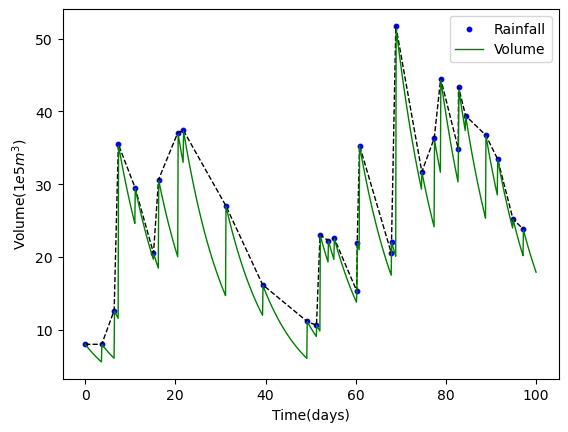
\includegraphics[width=0.45\textwidth]{rainfall.png}
  \caption{}
\end{figure}
\end{frame}

\section{Risque d’inondation}
\begin{frame}{Risque d’inondation}
    Problème du contrôle de risque d’inondation : trouver $x^\ast$ t.q.
    \[\P(X>x^\ast)\le \alpha,\ \alpha=10^{-6}.\]
    \begin{itemize}
        \item Pour un certain $T$ : $X=X_T$
        \item Pour le volume maximal pendant $[0,T]$ : $X=\max_{0\le s\le T}X_s$
    \end{itemize}
    \pause
    \textbf{Trois approches :}
    \begin{itemize}
        \item L'algorithme de Monte-Carlo naïf
        \item Importance Sampling
        \item L'algorithme de la dernière particule
    \end{itemize}
\end{frame}

\begin{frame}{Monte-Carlo naïf}
    \textbf{Idée} : simuler $N$ trajectoires $(X_i)$ de $X$ $\Longrightarrow$ prendre le quantile empirique
    \[\hat{q}_{1-\alpha} = \inf\{x\in \mathbb{R}:\hat{F}_N(x)\geq 1-\alpha\},\quad \hat{F}_N(x) = \frac{1}{N}\sum_{i=1}^N \mathbf{1}_{X_i\leq x}.\]
    Si on trie les valeurs de $X_i$ : $X_{(1,N)}\leq X_{(2,N)}\leq \cdots \leq X_{(N,N)}$, 
\[\hat{q}_{1-\alpha} = X_{(\lceil N(1-\alpha)\rceil,N)}.\]
\pause
\begin{itemize}
    \item Facile à implémenter : baseline pour les autres algorithmes
    \item Ne peut que traiter les cas où $\alpha$ n'est pas très petit
\end{itemize}
\end{frame}

\begin{frame}{Importance Sampling}
    \textbf{Idée :} changer vers une loi qui est plus «dense» autour du $q_{1-\alpha}$.
    Rappel : $A_t=\sum_{i=1}^{N_t}U_i$ est un processus de Poisson composé

    \vspace{5pt}
    
    \textbf{Transformation de Esscher :} Pour $f$ mesurable, $g$ fonction appliquée sur le trajectoire de $A_t$ :
    \[\E[g(A_t)]\approx \exp((\lambda_f-\lambda)T) \frac{1}{M}\sum_{i=1}^M g(A_t^{(i)})\exp\left(-\sum_{i=1}^{N_t^{(i)}}f(U_i^{(i)})\right),\]
    où $\lambda_f = \lambda \E[e^{f(U)}]$ et $\displaystyle \nu_f(du)=\frac{e^{f(u)}\nu(du)}{\E[e^{f(U)}]}$, $(A_t^{(i)})$ est une suite des processus de Poisson composé sous la mesure $(\lambda_f,\nu_f)$.
\end{frame}

\begin{frame}{Importance Sampling}
    \textbf{But} : estimer $q_{1-\alpha}$
    \[\E[g(A_t)]\approx \exp((\lambda_f-\lambda)T) \frac{1}{M}\sum_{i=1}^M g(A_t^{(i)})\exp\left(-\sum_{i=1}^{N_t^{(i)}}f(U_i^{(i)})\right)\]
    Soit $g(A_t)=\mathbf{1}_{X(A_t)>x^\ast}$, où 
    \begin{itemize}
        \item $X(A_t)=\max_{0\le s\le T}X_s(A_t)$ pour le volume maximal
        \item $X(A_t)=X_T(A_t)$ pour le volume en temps $T$
    \end{itemize}
    Il suffit de trouver $x^\ast$ t.q. $\E[g(A_t)]=\alpha$.
\end{frame}

\begin{frame}{Importance Sampling}
    \[\exp((\lambda_f-\lambda)T) \frac{1}{M}\sum_{i=1}^M \mathbf{1}_{X(A_t^{(i)})>x^\ast}\exp\left(-\sum_{i=1}^{N_t^{(i)}}f(U_i^{(i)})\right)\approx\alpha \]
\begin{algorithm}[H]
\begin{algorithmic}[1]
\State $X_n\leftarrow $ list of $X(A_t^{(i)})$ for $i=1,\cdots, M$
\State $V_n\leftarrow$ list of $\exp\left(-\sum_{i=1}^{N_t^{(i)}}f(U_i^{(i)})\right)$ for $i=1,\cdots, M$
\State $indices \leftarrow argsort(X_n)$; $idx\leftarrow 0;\ sum\leftarrow 0$
\While{$sum<\alpha M\exp(-(\lambda_f-\lambda)T)\ \&\ idx<M$}
\State $sum \leftarrow sum+ V_n[indices[idx]]; $ $idx ++$
\EndWhile 
\State $x^\ast\leftarrow  V_n[indices[idx]]$
\end{algorithmic}
\caption{Algorithme pour trouver $x^\ast$}
\end{algorithm}
\end{frame}

\begin{frame}{Importance Sampling}
    \textbf{Question :} comment choisir $f$ ?

    \vspace{5pt}
    
    Choix naturel : $f(u)=\sigma u+\beta$
    \begin{itemize}
        \item $\sigma>0$ : augmenter à la fois la densité et la fréquence des pluies
        \item $\beta>0$ : augmenter la fréquence des pluies
    \end{itemize}
    On peut montrer qu'un choix candidat est $\beta=0$, $\sigma$ la solution de
    \[-\sigma \phi_A'(\sigma)+\phi_A(\sigma)=\log(\alpha),\]
\[\phi_A(\sigma)=\lambda T(M_U(\sigma)-1),\ M_U(\sigma)=b\frac{\delta_1}{\delta_1-\sigma}+(1-b)\frac{\delta_2}{\delta_2-\sigma}.\]
\end{frame}


\begin{frame}{Algorithme de la dernière particule}
    \textbf{Idée :} renouveler la valeur minimale d'une suite de particules selon la loi de $(X|X>L)$ où $L=\min(X_i)$. \pause

    \textbf{Initialisation :} générer $(X_1^1,\dots, X_n^1)$ i.i.d. selon la loi de $X$. 

    Par récurrence, étant donné $(X_1^j,\dots,X_n^j)$ pour $j\geq 1$, on note $L_j=\min(X_1^j,\dots,X_n^j)$, et va construire $(X_1^{j+1},\dots,X_n^{j+1})$.
    
    Pour $1\leq i\leq n$,
    \begin{itemize}
        \item si $X_i^j>L_j$, alors $X_i^{j+1}=X_i^j$,
        \item si $X_i^j=L_j$, alors on génère $X_i^{j+1}$ selon la loi $(X|X>L_j)$ indépendamment.
    \end{itemize}
    
\end{frame}

\begin{frame}{Algorithme de la dernière particule}

    \textbf{Règle d'arrêt :} répéter $\displaystyle j_n = \left\lceil\frac{\log \alpha}{\log(1-1/n)}\right\rceil$ fois, le résultat est alors $\hat q_{n}=L_{j_n}$.
    
    \begin{algorithm}[H]
\begin{algorithmic}[1]
\State $X_N \gets $ list of $X(A_t^{(i)})_{1\leq i\leq N}$
\For {$\_ \gets 1$ \textbf{to} $j_n$}
    \State $L \gets \min(X_N)$
    \State $indices \gets \text{argwhere}(X_N == L)$
    \While{$index$ \textbf{in} $indices$}
        \State $X_N[index]\gets \text{get\_a\_new\_one}(L)$
    \EndWhile
\EndFor
\State $\hat q_n\gets L$
\end{algorithmic}
\caption{Algorithme pour obtenir $\hat q_n$}
\end{algorithm}

\end{frame}

\begin{frame}{Algorithme de la dernière particule}
\textbf{Question :} comment générer un échantillon indépendant selon la loi $(X|X>L)$ ?\pause

Rappeler que $X_t$ est obtenu du processus de Poisson composé $A_t$, il suffit alors de renouveler $A_t$ par l'algorithme de coloriage :\pause

\begin{itemize}
    \item garder chaque saut avec probabilité $p\in [0,1]$ de manière indépendante des autres, obtenir et noter $N_t^{(p)}$,
    \item calculer $qU_i+(1-q)V_i$ pour un point de saut gradé $i$, où $q\in[0,1]$ et $V_i\sim \nu$ indépendant de $U_i$, obtenir $A_t^{(p)}$,
    \item simuler un autre processus composé indépendant de paramètre $(1-p)\lambda$, noter $\bar{A}_t^{(1-p)}$, conclure en sommant $A_t^{(p)}$ et $\bar{A}_t^{(1-p)}$.
\end{itemize}

On veut répéter ce calcul plusieurs fois, en acceptant si le nouveau $\tilde{X}>L$, en refusant sinon.  
    
\end{frame}

\begin{frame}{Algorithme de la dernière particule}
        \begin{algorithm}[H]
\begin{algorithmic}[1]
\Require $N_t$ list of $T_i$, $U$ list of $U_i$, $p$ and $q$.
\For {$\_ \gets 1$ \textbf{to} $M$}
\State $Unif \gets \text{Unif of length } N_t$; $indices\gets \text{argwhere}(Unif < p)$
\State $N_t^{(p)}, U^{(p)}\gets N_t[indices], U[indices]$
\State $V \gets$ list of $\nu\text{ of length } N_t^{(p)}$; $U^{(p)}\gets qU^{(p)}+(1-q)V$
\State $\bar{N}_t^{(1-p)}\gets$ Poisson distribution of parametre $(1-p)\lambda$
\State $\bar{U}^{(1-p)}\gets$ list of $\nu\text{ of length } \bar{N}_t^{(1-p)}$
\State $\tilde{N}_t, \tilde{U}\gets N_t^{(p)}\cup \bar{N}_t^{(1-p)}, U^{(p)}\cup \bar{U}^{(1-p)}$
\If {$X(\tilde{A}_t)>L$}
\State $N_t,U\gets \tilde{N_t},\tilde{U}$
\EndIf
\EndFor
\end{algorithmic}
\caption{Algorithme pour obtenir un nouveau $\tilde{A}_t$}
\end{algorithm}
\textbf{Question :} comment choisir $p$, $q$ et $M$ ?
\end{frame}

\begin{frame}{Algorithme de la dernière particule}
    \textbf{Point clé :} devoir accepter un nombre suffisant de fois avant d'être considéré comme indépendant, sinon des erreurs se produiront, mais considérer aussi l'équilibre entre l'efficacité et l'exactitude. \pause

    Trois approches pour réaliser cet algorithme dans la pratique :
    \begin{itemize}
        \item fixer le nombre d'itérations $M$,
        \item augmenter le nombre d'itérations $M$ pendant l'exécution,
        \item fixer le nombre d'acceptations.
    \end{itemize} \pause

    Pour la sélection de $p$ et $q$, qui dépend en fait de $M$ et $\tilde M$, voir l'annexe du rapport.

    \textbf{Idée :} montrer les intervalles de confiance à différents $p$ et $q$ lorsque $\alpha$ n'est pas trop petit, comparés aux intervalles de confiance de Monte-Carlo naïf.
\end{frame}

\section{Simulation numérique}
\begin{frame}{Paramètres physiques}
    On met l'unité de temps comme $1$ an et l'unité de volume comme $10^5m^3$, et
    \begin{itemize}
        \item $r=1$, $T=1$, et il pleut $\lambda=70$ fois par an,
        \item $\delta_1=0.07$ et $\delta_2=0.7$, où son unité est $(10^5m^3)^{-1}$ et l'inverse de $\delta_i$ montre le volume moyen d'une seule pluie,
        \item la proportion $b=0.1$, i.e. seule une sur dix est une grande pluie,
        \item le quantile $\alpha=10^{-6}$.
    \end{itemize}
\end{frame}
\begin{frame}{Calcul de $x_0$}
On veut que $x_0$ soit <<l'état stationnaire>> pour que ce soit compatible avec le processus physique, i.e. le flux d'eau entrant et sortant est presque équilibré pendant assez longtemps.\pause

Pour un petit temps $\Delta t$, le flux sortant est $-(r x_0)\Delta t$ alors que le flux entrant est $\mathbb E[\nu](\lambda\Delta t)$. Pour que $x_0$ soit l'état stationnaire, on a forcément que  $-rx_0+\lambda{\mathbb E[\nu]}=0$, d'où
\[x_0=\frac{\lambda}{r}\left(\frac{b}{\delta_1}+\frac{1-b}{\delta_2}\right)=190.\]
    
\end{frame}
\begin{frame}{Estimation du quantile $q_{0.99}$}
    \textbf{But :} Comparer les trois approches; vérifier l'exactitude des implémentations
    \begin{figure}
        \centering
        \includegraphics[scale=0.5]{1-1.png}
        \caption{10 expériences sont faits indépendamment, err $=\max-\min$}
        \label{fig:enter-label}
    \end{figure}
\end{frame}

\begin{frame}{Estimation du quantile $q_{0.99}$}
\begin{table}[h!]
    \centering
    \begin{tabular}{|l|c|c|c|}
        \hline
        & \textbf{time cost (s)} & \textbf{mean ($10^5m^3$)} & \textbf{err} \\
        \hline
        Monte-Carlo naïf       &      1.0         &       330.2       &     1.9       \\
        \hline
        importance sampling   &      1.0         &        331.0      &     1.0       \\
        \hline
        last particle         &       13.7        &      331.9        &      3.1      \\
        \hline
    \end{tabular}
\end{table}
\begin{itemize}
    \item les trois algorithmes donnent le même résultat
    \item importance sampling a une variance et un coût plus petits
    \item l'algorithme de la dernière particule nous permet d'obtenir une estimation pour la distribution après la volume critique $x^\ast$ : $p(x|x>x^\ast)$
\end{itemize}
\end{frame}

\begin{frame}{Estimation du quantile $q_{0.99}$}
    \begin{figure}
        \centering
        \includegraphics[scale=0.5]{1-2.png}
        \caption{La distribution $p(x|x>q_{0.99})$ estimée par l'algorithme de la dernière particule.}
    \end{figure}
\end{frame}

\begin{frame}{Estimation du quantile $q_{1-10^{-6}}$}
MC naïf, Importance sampling avec $N=100,000$.\\
L'algorithme de la dernière particule avec $N=1,000$, $M=30$, on demande de plus qu'il y a au moins $M/2$ acceptations.
    \begin{figure}
        \centering
        \includegraphics[scale=0.5]{output 0.000001.png}
    \end{figure}
\end{frame}

\begin{frame}{Conclusion}
    Nous avons réussi à simuler le risque d'inondation, qui est un effet un événement rare, avec deux approches différentes : l'importance sampling et l'algorithme de la dernière particule. 
    \begin{itemize}
        \item l'importance sampling est très efficace pour ce problème et donne un résultat assez précis.
        \item l'algorithme de la dernière particule est plus flexible et nous permet aussi d'estimer la distribution dépassant le niveau critique.
        \item les choix des hyperparamètres dans ces deux algorithmes jouent un rôle crucial.
    \end{itemize}
\end{frame}

\begin{frame}{Travaux de future}
    \begin{itemize}
        \item Etudier l'effet d'un $\beta\ne 0$. Nous avons utilisé un transformation de $f(x)=\sigma x+\beta$ avec $\beta =0$ dans importance sampling. En fait, prendre un $\beta>0$ a un impact similaire que prendre $\sigma>0$.
        \item Comprendre plus l'impact de $p,q$ dans l'algorithme de la dernière particule, surtout d'un point de vue théorique.
    \end{itemize}
\end{frame}
\end{document}